\providecommand{\main}{.}

\documentclass{report} % We use report to allow for chapers etc...
\usepackage{etoolbox}
\usepackage{geometry} % More rich support for page layout.
\geometry{
	a4paper,
	total={190mm,260mm},
	left=10mm,
	top=20mm,
}

\ifdef{\main}{}{
	\providecommand{\main}{/Users/lucacappelletti/github/various-notes/Polimi/Meccanica}
}
\usepackage{silence}
%Disable all warnings issued by latex starting with "You have..."
\WarningFilter{latex}{You have requested package}
\WarningFilter{latex}{There were undefined references}
\WarningFilter{latexfont}{Size substitutions with differences}
\WarningFilter{latexfont}{Font shape}
\WarningFilter{latex}{Command}
\WarningFilter{biblatex}{Using fall-back BibTeX(8)}
\WarningFilter{biblatex}{Please (re)run BibTeX on the file(s)}
\WarningFilter{auxhook}{Cannot patch}
\WarningFilter{glossaries}{No \printglossary or \printglossaries found.}

\usepackage{amsmath,amsthm,amsfonts,amssymb}
\usepackage{array}   % for \newcolumntype macro
\newcolumntype{L}{>{$}l<{$}} % automaticall apply mathmode to column

\theoremstyle{definition} % Sets the theorem style without italic
\usepackage{bm} % To have bold vectors

\usepackage{fp}
\usepackage{xparse}

\usepackage{iftex} % Used for if
\ifLuaTeX
	\directlua{pdf.setcompresslevel(9)}
	\directlua{pdf.setobjcompresslevel(2)}
	\directlua{pdf.setminorversion(5)}
	\usepackage{shellesc}
	\usepackage{polyglossia}
	\setotherlanguage{english}
	\setdefaultlanguage{italian}
	\usepackage{fontspec}
	\usepackage{luacode} % Used to script stuff
\else
	\usepackage[utf8]{inputenc} % This allows for utf support.
	\usepackage[english, italian]{babel}   % Set up supported languages. Last one is default.
\fi

\usepackage[T1]{fontenc}  % Defines true type fonts

\usepackage[x11names,table]{xcolor} % To highlight text or color tables

\usepackage{emptypage} % When a page is empty, Latex won't generate page number or other page elements.

\usepackage{multicol} % For the possibility of using columns with  \begin{multicols}{n}.
\usepackage[colorlinks=true,urlcolor=blue,pdfpagelabels,hyperindex=false]{hyperref}  % Enable table of contents and links.
\usepackage{microtype} % for automatic micro fitting of characters
\usepackage{centernot} % Adds not symbol on any math symbol.

\usepackage{framed}
\usepackage{float} % to enable floating graphics
\usepackage[style=authoryear,sorting=ynt, backend=bibtex]{biblatex} % Package to handle the bibliography
\usepackage{subfiles} % To use subfiles without cruxifying saints

\usepackage{parskip} % To leave spaces in paragraphs without using \\
\usepackage{soul} % To cancel text with a line using the commant \st, to underline text and highlight.

\usepackage{xfrac} % To allow for sideways fractions
\usepackage[cache=true]{minted} % For highlighting code
\usepackage[algoruled,linesnumbered,titlenumbered]{algorithm2e} % To highlight pseudocode
\definecolor{mintedbackground}{rgb}{0.95,0.95,0.95}
\setminted{
	bgcolor=mintedbackground,
	fontfamily=tt,
	linenos=true,
	numberblanklines=true,
	numbersep=5pt,
	gobble=0,
	frame=leftline,
	framerule=0.4pt,
	framesep=2mm,
	funcnamehighlighting=true,
	tabsize=4,
	obeytabs=false,
	mathescape=false
	samepage=false, %with this setting you can force the list to appear on the same page
	showspaces=false,
	showtabs =false,
	texcl=false,
}

% CDQUOTES HAS TO BE LOADED AFTER THE MINTED
\usepackage{csquotes} % Package required by babel AND polyglossia.

%%%%%%%%%%%%%%%%%%%%%%%%%
% GRAPHICAL EXTRAVAGANZA %
%%%%%%%%%%%%%%%%%%%%%%%%%

\usepackage{pgfplots} % to draw 3d graphs
\pgfplotsset{compat=1.14}
\usepackage{tikz}
\usepackage{tikz-qtree}
\usepackage{relsize}
\usepackage{circuitikz}
\usepackage{bodegraph}
\usepackage{adigraph}

\ctikzset{tripoles/mos style/arrows}
\ctikzset{tripoles/pmos style/emptycircle}
\usetikzlibrary{shapes,arrows,calc,positioning,matrix}
\usepgfplotslibrary{external}

\pgfplotsset{samples=60,shader=interp,grid=both}

\usepackage{paralist} % For compacted enumerations
\usepackage[automake,style=long,nonumberlist,toc,acronym,nomain]{glossaries} % for glossaries and acronyms
\makeglossaries % Enables the package above

\usepackage{imakeidx} % instead of makeidx, so you don't need to run MakeIndex
\makeindex[program=makeindex,columns=2,intoc=true,options={-s ../../general/pyro.ist}] % Enables the package above
\indexsetup{firstpagestyle=empty, othercode=\small} % No page number in the first page of analytical index

\usepackage{fourier} % For icons such as \bomb, \noway, \danger and various others. For more info, go here: http://ctan.mirror.garr.it/mirrors/CTAN/fonts/fourier-GUT/doc/latex/fourier/fourier-orns.pdf
\usepackage{marvosym} % For icons such as \Cross

\renewcommand*{\arraystretch}{1.25} % Stretching arrays

\usepackage{sectsty} % Styles sectional headers
\usepackage{fancyhdr} % This allows for the headings in the chapters
\pagestyle{fancy} % This activates it
\usepackage[avantgarde]{quotchap} % Custom style for chapters

\makeatletter
\renewcommand{\@makechapterhead}[1]{%
	%\chapterheadstartvskip%
	{\size@chapter{\sectfont\raggedleft
				{\chapnumfont
					\ifnum \c@secnumdepth >\m@ne%
						\if@mainmatter\thechapter\else\phantom{\thechapter}%
						\fi\else\phantom{\thechapter}\fi
					\par\nobreak}%
				{\raggedleft\advance\leftmargin10em\interlinepenalty\@M #1\par}}
			\nobreak\chapterheadendvskip}}
\makeatother



%%%%%%%%%%%%%%%%%%%%%%%%%%%%%%%%%%%%%%%%%%%%%%%%%%%%%%%%%

\usepackage[shortlabels]{enumitem} % For a todo check list
\newlist{todolist}{itemize}{2} % For a  todo check list
% \setlist{nolistsep}
\setlist[todolist]{label=$\square$}  % For a todo check list



%%%%%%%%%%%%%%%%%%%%%%%%%
% LUATEX CODE %
%%%%%%%%%%%%%%%%%%%%%%%%%

\ifLuaTeX
	\begin{luacode}
function fileExists(name)
   local f=io.open(name,"r")
   if f~=nil then io.close(f) return true else return false end
end

--[[We define 5 levels of recursive attempts]]
local levels = 10

--[[The expected file name is the following]]
local target = '/general/packages.tex'
deapness = '../'

for i=levels,1,-1 do
    --[[if we have a path that exists we exit]]
    if fileExists(deapness..target) then break end

    --[[We increase the path one level up]]
    deapness = '../'..deapness
end
\end{luacode}
	\directlua{dofile(deapness.."/general/lua/metadataLoader.lua")}
	\directlua{dofile(deapness.."/general/lua/languageSwitch.lua")}
	\directlua{dofile(deapness.."/general/lua/highlight.lua")}

	% THE FOLLOWING IS AN EXAMPLE ON HOW TO DEFINE A LUA COMMAND
	% \def\command{\directlua{dofile(deapness.."/general/lua/fileName.lua")}}
	% \command
\else
	% Lua not enabled
	\renewcommand{\chaptername}{Capitolo}
\renewcommand{\contentsname}{Indice}
\newtheorem{theorem}{Teorema}[section]
\newtheorem{corollary}{Corollario}[theorem]
\newtheorem{lemma}[theorem]{Lemma}
\newtheorem{definition}[theorem]{Definizione}
\fi

\let\oldtextbf\textbf % This is a backup for options may edit \textbf
\let\oldtextit\textit % This is a backup for options may edit \textit
\let\oldemph\emph % This is a backup for options may edit \emph

%
% THE FOLLOWING CODE ALLOWS FOR ROMAN NUMBERS
%

\makeatletter
\newcommand*{\rom}[1]{\expandafter\@slowromancap\romannumeral #1@}
\makeatother

%
% THE FOLLOWING CODE WRAPS THEOREMS IN A GRAY BOX
%
\colorlet{shadecolor}{gray!10}
\let\oldTheorem\theorem
\renewenvironment{theorem}{\begin{shaded}\begin{oldTheorem}}{\end{oldTheorem}\end{shaded}\ignorespacesafterend
}

\let\oldDefinition\definition
\renewenvironment{definition}{\begin{shaded}\begin{oldDefinition}}{\end{oldDefinition}\end{shaded}\ignorespacesafterend
}

\let\oldCorollary\corollary
\renewenvironment{corollary}{\begin{shaded}\begin{oldCorollary}}{\end{oldCorollary}\end{shaded}\ignorespacesafterend
}

\let\oldProposition\proposition
\renewenvironment{proposition}{\begin{shaded}\begin{oldProposition}}{\end{oldProposition}\end{shaded}\ignorespacesafterend
}

%
% THE FOLLOWING CODE ADDS BOLD TO THE THEOREM NAME
%

\makeatletter
\def\th@plain{%
	\thm@notefont{}% same as heading font
	\itshape % body font
}
\def\th@definition{%
	\thm@notefont{}% same as heading font
	\normalfont % body font
}
\makeatother

\definecolor {processblue}{cmyk}{0.96,0,0,0}
\def\checkmark{\tikz\fill[scale=0.4](0,.35) -- (.25,0) -- (1,.7) -- (.25,.15) -- cycle;}

\newcommand{\error}[1]{
	\textcolor{red!90}{#1}
}

\newcommand{\bash}[1]{
	\immediate\write18{#1}
}

\newcommand{\dddgraph}[9]{
	%#1-> X-axis label
	%#2-> Y-axis label
	%#3-> Min x value
	%#4-> Max x value
	%#5-> Min y value
	%#6-> Max y value
	%#7-> Min z value
	%#8-> Area of definition, defined as boolean expression
	%#9-> function
	\begin{tikzpicture}
		\begin{axis}[
				xlabel=$#1$,
				width=\textwidth,
				ylabel=$#2$,
				zlabel=$z$,
				domain=#3:#4,
				y domain=#5:#6,
				xmin=#3,
				xmax=#4,
				ymin=#5,
				ymax=#6
			]
			\addplot3[opacity=0.7,color=gray]{#8?#7:NaN};
			\addplot3[surf, unbounded coords=jump]{#8?#9:NaN};
		\end{axis}
	\end{tikzpicture}
}

\newcommand{\xygraph}[7]{
	%#1-> Min x value
	%#2-> Max x value
	%#3-> Min y value
	%#4-> Max y value
	%#5-> Min z value
	%#6-> Area of definition, defined as boolean expression
	%#7-> function
	\dddgraph{x_1}{x_2}{#1}{#2}{#3}{#4}{#5}{#6}{#7}
}

\newcommand{\posxygraph}[5]{
	%#1-> Max x value
	%#2-> Max y value
	%#3-> Min z value
	%#4-> Area of definition, defined as boolean expression
	%#5-> function
	\xygraph{0}{#1}{0}{#2}{#3}{#4}{#5}
}

\newcommand{\posxyzgraph}[4]{
	%#1-> Max x value
	%#2-> Max y value
	%#3-> Area of definition, defined as boolean expression
	%#4-> function
	\posxygraph{#1}{#2}{0}{#3}{#4}
}

%%%%%%%%%%%%%%%%%%%%%%%%%
% EXTERNAL FILES %
%%%%%%%%%%%%%%%%%%%%%%%%%

\NewDocumentCommand{\smartif}{m m O{} O{}}{
  %
  % #1 -> The first part of the equation
  % #2 -> The second part of the equation
  % #3 (optional) -> Stuff to do if it is true
  % #4 (optional) -> Stuff to do if it is false
  %
  % USAGE EXAMPLE:
  % I want to write concatenated ifs without blaspheming the name of the great one, Cthulhu.
  %
  %
  % \def{\cthulhuislord}{0}
  % \def{\true}{1}
  %
  % \smartif{\cthulhuislord}{\true}[
  %  Yes, cthulhu is lord
  %  ][
  %  No, I think it is a bit unstable
  %  ]
  %
  \FPifeq{#1}{#2}
  #3
  \else
  #4
  \fi
}
\NewDocumentCommand{\FPceil}{m m}{
  %
  % #1 -> number to assign
  % #2 -> number to ceil
  %
  \FPadd{\numberplusone}{#2}{1}
  \FPfloor{#1}{\numberplusone}
}
\NewDocumentCommand{\FPfloor}{m m}{
  %
  % #1 -> number to assign
  % #2 -> number to floor
  %
  \FPtrunc{#1}{#2}{0}
}

\usepackage{graphicx} % for images and generally graphics
\usepackage{caption} % enabling of nice captions
\usepackage{subcaption} % and subcaptions of images
\graphicspath{ {\main/images/} } % We'll put all the images in the folder "images"

\setlength{\intextsep}{3pt plus 2pt minus 2pt}

%%%%%%%%%%%%%%%%%%%%%%%%%%%%%%%%%%%%%%%%%%%%%%%%%%%%%%%%%
% THE FOLLOWING CENTERS ALL FLOATING ITEMS BY DEFAULT   %
%%%%%%%%%%%%%%%%%%%%%%%%%%%%%%%%%%%%%%%%%%%%%%%%%%%%%%%%%

\makeatletter
\g@addto@macro\@floatboxreset\centering
\makeatother

\makeatletter
\apptocmd\subcaption@minipage{\centering}{}{}
\makeatother
\makeatletter
\providecommand*\setfloatlocations[2]{\@namedef{fps@#1}{#2}}
\makeatother
\setfloatlocations{figure}{H}
\setfloatlocations{table}{H}
\NewDocumentCommand{\smartFigureWidth}{m m m m m}{
  %
  % #1 -> Current remaining figures
  % #2 -> Last row figures number
  % #3 -> Normal Width
  % #4 -> Last row width
  % #5 -> Variable to assign
  %
  \FPifeq{#1}{#2}%
  \FPset{#5}{#4}
  \else%
  \FPsub{#1}{#1}{1}
  \FPset{#5}{#3}
  \fi%
}
\NewDocumentCommand{\fig}{m m g g g g O{1} g O{1}}{%
  %
  % PARAMETERS MEANING
  %
  % #1 (Mandatory)                     -> First figure
  % #2 (Mandatory)                     -> Second figure
  % #3 (Optional, with curly braces)   -> Third figure
  % #4 (Optional, with curly braces)   -> Forth figure
  % #5 (Optional, with curly braces)   -> Fifth figure
  % #6 (Optional, with curly braces)   -> Sixth figure
  % #7 (Optional, with squared braces) -> Maximum width, based on percentage of \textwidth.
  % #8 (Optional, with curly braces) -> Elements to add at the bottom, such as labels of caption for the group
  % #9 (Optional, with squared braces) -> Maximum number of figures per row
  %
  %--------------------------------------
  %
  % USAGE EXAMPLES
  %
  % \fig{<content of figure 1 here>}{<content of figure 2 here>}{...}[Width I want]{<elements for bottom, such as caption>}
  %
  % IMPORTANT: For having the group caption evaluated correctly, one must insert also the width.
  %
  % Example with 1 figure:
  %
  % I want to show a kebab, with a width of 0.5 of the textwidth and as caption and label ``kebab''.
  %
  % \fig{\includegraphics{kebab.jpg}}[0.5]{
  %   \caption{kebab}
  %   \label{kebab}
  % }
  %
  % Example with 2 figures:
  %
  % I want to show two diagrams, one 3d and the projection, width each one occuping 0.5 of textwidth and with common label and caption ``graphs''.
  %
  % \fig{\includegraphics{graph3d.jpg}}{\includegraphics{graph2d.jpg}}[1]{
  %   \caption{graphs}
  %   \label{graphs}
  % }
  %
  %--------------------------------------
  %
  \FPset{\figuresNumber}{2}
  \IfValueT{#3}{
    \FPadd{\figuresNumber}{\figuresNumber}{1}
    \IfValueT{#4}{
      \FPadd{\figuresNumber}{\figuresNumber}{1}
      \IfValueT{#5}{
        \FPadd{\figuresNumber}{\figuresNumber}{1}
        \IfValueT{#6}{
          \FPadd{\figuresNumber}{\figuresNumber}{1}
        }
      }
    }
  }
  \FPset{\rowsNumber}{#9}
  \FPset{\remainingFigures}{\figuresNumber}
  \FPdiv{\figuresPerRow}{\figuresNumber}{\rowsNumber}
  \FPceil{\figuresPerRow}{\figuresPerRow}
  \FPsub{\fullRowsNumber}{\rowsNumber}{1}
  \FPmul{\flooredFiguresNumber}{\fullRowsNumber}{\figuresPerRow}
  \FPsub{\lastRowFiguresNumber}{\figuresNumber}{\flooredFiguresNumber}
  % end of ceil
  \FPdiv{\figureWidth}{#7}{\figuresPerRow}
  \FPdiv{\lastRowWidth}{#7}{\lastRowFiguresNumber}
  %Applying margin coefficient
  \FPset{\marginCoefficient}{0.9}
  \FPmul{\figureWidth}{\figureWidth}{\marginCoefficient}
  \FPmul{\lastRowWidth}{\lastRowWidth}{\marginCoefficient}
  %
  \smartif{\figuresNumber}{\one}[
    \begin{figure}
      \scalebox{\figureWidth\textwidth}{#1}
      \IfValueT{#8}{
        #8
      }
    \end{figure}
  ][
    \begin{figure}
      \smartFigureWidth{\remainingFigures}{\lastRowFiguresNumber}{\figureWidth}{\lastRowWidth}{\smartWidth}
      \begin{subfigure}{\smartWidth\textwidth}
        #1
      \end{subfigure}
      \smartFigureWidth{\remainingFigures}{\lastRowFiguresNumber}{\figureWidth}{\lastRowWidth}{\smartWidth}
      \begin{subfigure}{\smartWidth\textwidth}
        #2
      \end{subfigure}
      \IfValueT{#3}{
        \smartFigureWidth{\remainingFigures}{\lastRowFiguresNumber}{\figureWidth}{\lastRowWidth}{\smartWidth}
        \begin{subfigure}{\smartWidth\textwidth}#3\end{subfigure}
      }
      \IfValueT{#4}{
        \smartFigureWidth{\remainingFigures}{\lastRowFiguresNumber}{\figureWidth}{\lastRowWidth}{\smartWidth}
        \begin{subfigure}{\smartWidth\textwidth}#4\end{subfigure}
      }
      \IfValueT{#5}{
        \smartFigureWidth{\remainingFigures}{\lastRowFiguresNumber}{\figureWidth}{\lastRowWidth}{\smartWidth}
        \begin{subfigure}{\smartWidth\textwidth}#5\end{subfigure}
      }
      \IfValueT{#6}{
        \smartFigureWidth{\remainingFigures}{\lastRowFiguresNumber}{\figureWidth}{\lastRowWidth}{\smartWidth}
        \begin{subfigure}{\smartWidth\textwidth}#6\end{subfigure}
      }
      \IfValueT{#8}{
        #8
      }
    \end{figure}
  ]

}%
\DeclareMathOperator{\var}{Var}
\DeclareMathOperator{\conv}{conv}
\DeclareMathOperator*{\argmin}{argmin}
\DeclareMathOperator*{\argmax}{argmax}
\DeclareMathOperator*{\mcd}{mcd}
\DeclareMathOperator*{\mcp}{mcp}
%\DeclareMathOperator* this one allows to create environment that behave like sum or min

\newcommand{\crs}{\text{\Cross}}

\newcommand{\bra}[1]{\left\langle#1\right\rvert}
\newcommand{\ket}[1]{\left\lvert#1\right\rangle}
\newcommand{\braket}[2]{\left\langle#1\delimsize\vert#2\right\rangle}

\newcommand{\ceil}[1]{\left\lceil#1\right\rceil}
\newcommand{\floor}[1]{\left\lfloor#1\right\rfloor}

\newcommand{\abs}[1]{\left\lvert#1\right\rvert}
\newcommand{\norm}[1]{\left\lVert#1\right\rVert}
\newcommand{\rnd}[1]{\left(#1\right)}
\newcommand{\sqr}[1]{\left[#1\right]}
\newcommand{\crl}[1]{\left\{#1\right\}}
\newcommand{\arity}[1]{\#\crl{#1}}

\let\oldbm\bm
\renewcommand{\bar}{\overline}
\renewcommand{\bm}[1]{\oldbm{\underline{#1}}}
\newcommand{\matr}[1]{\boldsymbol{#1}}
\newcommand{\bbm}[1]{\bar{\bm{#1}}}
\renewcommand{\geq}{\geqslant}
\renewcommand{\leq}{\leqslant}

\def\zero{0}
\def\one{1}
\def\negative{-}
\def\positive{+}
\def\false{\zero}
\def\true{\one}
\newcommand{\R}{\mathbb{R}}
\newcommand{\Z}{\mathbb{Z}}
\newcommand{\N}{\mathbb{N}}
\newcommand{\bs}{\backslash}

\renewcommand{\O}[1]{\mathcal{O}\rnd{#1}}

\NewDocumentCommand{\gmr}{m}{%
    %
    % #1 -> Value to build gomory cut upon
    %
    \rnd{#1-\floor{#1}}
}


\NewDocumentCommand{\buildVectorAliases}{m O{#1}}{
    %
    % #1 -> Letter to use for aliases
    % #2 -> Symbol to use as output
    %
    \expandafter\newcommand\csname bm#1\endcsname{\bm{#2}}%
    \expandafter\newcommand\csname bm#1o\endcsname{{\bm{#2}^*}}%
    \expandafter\newcommand\csname bbm#1\endcsname{\bbm{#2}}%
    \expandafter\newcommand\csname bm#1t\endcsname{{\bm{#2}^T}}%
    \expandafter\newcommand\csname bbm#1t\endcsname{{\bbm{#2}^T}}%
}

\renewcommand{\a}{\alpha}
\newcommand{\w}{\omega}
\newcommand{\e}{\epsilon}

\buildVectorAliases{a}[\a]
\buildVectorAliases{w}[\w]
\buildVectorAliases{b}
\buildVectorAliases{c}
\buildVectorAliases{d}
\buildVectorAliases{h}
\buildVectorAliases{g}
\buildVectorAliases{p}
\buildVectorAliases{u}
\buildVectorAliases{v}
\buildVectorAliases{x}
\buildVectorAliases{y}
\buildVectorAliases{z}
\newacronym{fol}{FOL}{First Order Logic}
\def\hz{
	Hz
}
\def\db{
	dB
}
\NewDocumentCommand{\normal}{G{0} G{1}}{%
  \mathcal{N}\rnd{#1, #2}
}

\NewDocumentCommand{\prob}{m o G{} G{} G{}}{%
  %
  % #1 -> first term of probability
  % #2 (optional) -> operator beetween probabilities, defaults to conditioned probabilities.
  % #3 (optional) -> second term of probability, when conditioned
  % #4 (optional) -> subscript
  % #5 (optional) -> upscript
  %
  \ifblank{#3}{%
    \mathbb{P}_{#4}^{#5}\rnd{#1}
  }{%
    \IfNoValueTF{#2}{%
      \mathbb{P}_{#4}^{#5}\rnd{\left. #1 \;\right\rvert\; #3}
    }{%
      \mathbb{P}_{#4}^{#5}\rnd{#1\;#2\;#3}
    }
  }
}

\NewDocumentCommand{\mean}{m o G{} G{} G{}}{%
  %
  % #1 -> first term of mean
  % #2 (optional) -> operator beetween events, defaults to conditioned probabilities.
  % #3 (optional) -> second term of mean, when conditioned
  % #4 (optional) -> subscript
  % #5 (optional) -> upscript
  %
  \ifblank{#3}{%
    \mathbb{E}_{#4}^{#5}\rnd{#1}
  }{%
    \IfNoValueTF{#2}{%
      \mathbb{E}_{#4}^{#5}\rnd{\left. #1 \;\right\rvert\; #3}
    }{%
      \mathbb{E}_{#4}^{#5}\rnd{#1\;#2\;#3}
    }
  }
}

\NewDocumentCommand{\Var}{m o g}{%
  %
  % #1 -> first term of mean
  % #2 (optional) -> operator beetween events, defaults to conditioned probabilities.
  % #3 (optional) -> second term of mean, when conditioned
  %
  \IfNoValueTF{#3}{%
    \text{Var}\rnd{#1}
  }{%
    \IfNoValueTF{#2}{%
      \text{Var}\rnd{\left. #1 \;\right\rvert\; #3}
    }{%
      \text{Var}\rnd{#1\;#2\;#3}
    }
  }
}

\NewDocumentCommand{\tprob}{m o g}{%
  %
  % Alias of prob that textualizes the events.
  %
  \IfNoValueTF{#3}{%
    \prob{\text{#1}}
  }{%
    \IfNoValueTF{#2}{%
      \prob{\text{#1}}{\text{#3}}
    }{%
      \prob{\text{#1}}[#2]{\text{#3}}
    }
  }
}

\NewDocumentCommand{\bayes}{m m}{%
  %
  % #1 -> event X
  % #2 -> event Y
  %
  \prob{#1}{#2} &= \frac{\prob{#2}{#1}\prob{#1}}{
    \prob{#2}
  }%
}

\NewDocumentCommand{\tbayes}{m m}{%
  %
  % Textual alias for bayes
  %
  \bayes{\text{#1}}{\text{#2}}
}

\NewDocumentCommand{\totProb}{m m g g g g g g g}{%
  %
  % #1 (mandatory) -> event E
  % #2 (mandatory) -> event F_1
  % #3 (optional)  -> event F_2
  % #4 (optional)  -> event F_3
  % #5 (optional)  -> event F_4
  % #6 (optional)  -> event F_5
  % #7 (optional)  -> event F_6
  % #8 (optional)  -> event F_7
  % #9 (optional)  -> event F_8
  %
  \prob{#1} &= \prob{#1}{#2}\prob{#2}%
  \IfValueT{#3}{%
    +\prob{#1}{#3}\prob{#3}%
  }%
  \IfValueT{#4}{%
    +\prob{#1}{#4}\prob{#4}%
  }%
  \IfValueT{#5}{%
    +\prob{#1}{#5}\prob{#5}%
  }%
  \IfValueT{#6}{%
    +\prob{#1}{#6}\prob{#6}%
  }%
  \IfValueT{#7}{%
    +\prob{#1}{#7}\prob{#7}%
  }%
  \IfValueT{#8}{%
    +\prob{#1}{#8}\prob{#8}%
  }%
  \IfValueT{#9}{%
    +\prob{#1}{#9}\prob{#9}%
  }%
}

\NewDocumentCommand{\ttotProb}{m m g g g g g g g}{%
  \tprob{#1} &= \tprob{#1}{#2}\tprob{#2}%
  \IfValueT{#3}{%
    +\tprob{#1}{#3}\tprob{#3}%
  }%
  \IfValueT{#4}{%
    +\tprob{#1}{#4}\tprob{#4}%
  }%
  \IfValueT{#5}{%
    +\tprob{#1}{#5}\tprob{#5}%
  }%
  \IfValueT{#6}{%
    +\tprob{#1}{#6}\tprob{#6}%
  }%
  \IfValueT{#7}{%
    +\tprob{#1}{#7}\tprob{#7}%
  }%
  \IfValueT{#8}{%
    +\tprob{#1}{#8}\tprob{#8}%
  }%
  \IfValueT{#9}{%
    +\tprob{#1}{#9}\tprob{#9}%
  }%
}

\def\bayesTh{
  \begin{theorem}[Teorema di Bayes]
    Dati due eventi, $X$ e $Y$, con $\prob{Y}\neq0$, allora vale l'equazione:
    \begin{align*}
      \bayes{X}{Y}
    \end{align*}
    Dove:
    \begin{itemize}
      \item $\prob{X}{Y}$ è la probabilità condizionata rappresentante la verosimiglianza che l'evento $X$ avvenga dato che è avvenuto $Y$.
      \item $\prob{Y}{X}$ è la probabilità condizionata rappresentante la verosimiglianza che l'evento $Y$ avvenga dato che è avvenuto $X$.
      \item $\prob{X}$ è la probabilità a priori di $X$ ed è detta \textbf{probabilità marginale}.
      \item $\prob{Y}$ è la probabilità a priori di $Y$ e funge da costante di normalizzazione.
    \end{itemize}
  \end{theorem}
}
\def\formulaProbTot{
  \begin{definition}[Formula delle probabilità totali]
    Sia \((\Omega, \mathcal{F}, P)\) uno spazio di probabilità e \(F_1, F_2, \ldots, F_n \in \mathcal{F}\) una partizione finita di \(\omega\), \(\bigcup_{k=1}^n F_k = \Omega \) e \(F_h \cap F_k = \emptyset \) se \( h\neq k\), tale che \( \prob{F_k}>0\) per \(k=1,2,\dots,n\). Allora ogni evento \(E \in \mathcal{F}\) si ha:
    \[
      \prob{E} = \sum_{k=1}^n\prob{E}{F_k}\prob{F_k}
    \]
  \end{definition}

  \begin{corollary}[Corollario sulla media]
    \[
      \mean{E} = \sum_{k=1}^n \mean{E}{F_k}\prob{F_k}
    \]
  \end{corollary}
}
\providecommand{\main}{.}
\input{\main/../../general/packages.tex}
\usepackage{booktabs}
\begin{document}

\input{\main/../../general/title.tex}

{\hypersetup{hidelinks}
	\tableofcontents  % Generates the table of contents
}
\part{Dataset}
\chapter{Data points}
First we begin looking at the dataset, the distributions of the given metrics and the statistical analysis of these data points.

\section{Retrieving the dataset}
The dataset can be downloaded from \url{https://homes.di.unimi.it/valentini/ProgettoBioinformatica1718/data/}.

\section{Composition}
\subsection{Training dataset}
In the training dataset there are 981389 data points, each one comprised of 26 metrics. The first 356 are pathogenic and all the others are negative.

\subsection{Testing dataset}
In the test dataset there are 190189 data points, still each one comprised of 26 metrics. The first 40 are pathogenic and the following are negative.

\chapter{Metrics}
\section{How the graphs are realized}
All the graphs are in triples: positives, negatives and mixed. All the zeros are removed as in most metrics \textit{seemed} to indicate an unknown value.

\subsection{Metric sample distribution}
Are realized by calculating the frequencies and estimating the density distributions parameters via MLE.

\subsection{Plot graphs}
Are realized by sorting the values of the metric.

\subsection{Normalized plot graphs}
Are realized by sorting the values of the metric, with the domain and codomain normalized.

\clearpage
\section{CpGobsExp}
\subsection{Metric sample distribution}
The data points seem to follow a \textbf{Beta} distribution with the following parameters:

\begin{align*}
	\alpha   = 7.6689746880295795     & \qquad  \beta = 6778383.524935903       \\
	\text{loc} = -0.09826818916997124 & \qquad \text{scale} = 306278.3184506849
\end{align*}

\begin{figure}
	\includegraphics[width=\textwidth]{metrics_statistics/CpGobsExp}
	\caption{Sampling distribution of metric CpGobsExp}
\end{figure}
\subsection{Metric values}
\begin{figure}
	\includegraphics[width=\textwidth]{metrics_plot/CpGobsExp}
	\caption{Values of metric CpGobsExp}
\end{figure}

\clearpage
\section{CpGperCpG}
\subsection{Metric sample distribution}
The data points seem to follow a \textbf{Beta} distribution with the following parameters:

\begin{align*}
	\alpha   = 6.402175341881067      & \qquad  \beta = 97129163.31117742      \\
	\text{loc} = -0.05698922703576313 & \qquad \text{scale} = 4337764.42876015
\end{align*}
\begin{figure}
	\includegraphics[width=\textwidth]{metrics_statistics/CpGperCpG}
	\caption{Sampling distribution of metric CpGperCpG}
\end{figure}
\subsection{Metric values}
\begin{figure}
	\includegraphics[width=\textwidth]{metrics_plot/CpGperCpG}
	\caption{Values of metric CpGperCpG}
\end{figure}

\clearpage
\section{CpGperGC}
\subsection{Metric sample distribution}
The data points seem to follow a \textbf{Gaussian} distribution with the following parameters:

\begin{align*}
	\mean{X} = 0.4602356242601636 & \qquad \Var{X} = 0.15949294643574352
\end{align*}
\begin{figure}
	\includegraphics[width=\textwidth]{metrics_statistics/CpGperGC}
	\caption{Sampling distribution of metric CpGperGC}
\end{figure}
\subsection{Metric values}
\begin{figure}
	\includegraphics[width=\textwidth]{metrics_plot/CpGperGC}
	\caption{Values of metric CpGperGC}
\end{figure}

\clearpage
\section{DGVCount}
\subsection{Metric sample distribution}
The data points seem to follow a \textbf{Gamma} distribution with the following parameters:
\begin{align*}
	\alpha   = 0.20940038672579409    \qquad  \text{loc} = -1.1962983066939984e-30 \qquad \text{scale} = 1.2347090894162929
\end{align*}
\begin{figure}
	\includegraphics[width=\textwidth]{metrics_statistics/DGVCount}
	\caption{Sampling distribution of metric DGVCount}
\end{figure}
\subsection{Metric values}
\begin{figure}
	\includegraphics[width=\textwidth]{metrics_plot/DGVCount}
	\caption{Values of metric DGVCount}
\end{figure}

\clearpage
\section{DnaseClusteredHyp}
\subsection{Metric sample distribution}
The data points seem to follow a \textbf{Gamma} distribution with the following parameters:
\begin{align*}
	\alpha   = 0.4176887081406805    \qquad  \text{loc} = -3.362626207862299e-29 \qquad \text{scale} = 0.3676310948709975
\end{align*}
\begin{figure}
	\includegraphics[width=\textwidth]{metrics_statistics/DnaseClusteredHyp}
	\caption{Sampling distribution of metric DnaseClusteredHyp}
\end{figure}
\subsection{Metric values}
\begin{figure}
	\includegraphics[width=\textwidth]{metrics_plot/DnaseClusteredHyp}
	\caption{Values of metric DnaseClusteredHyp}
\end{figure}

\clearpage
\section{DnaseClusteredScore}
\subsection{Metric sample distribution}
The data points seem to follow \textbf{slightly} a \textbf{Beta} distribution with the following parameters:
\begin{align*}
	\alpha   = 0.2709657632937803     & \qquad  \beta = 0.44530002562349713      \\
	\text{loc} = -0.09309893086089688 & \qquad \text{scale} = 1.0930989308608972
\end{align*}

\begin{figure}
	\includegraphics[width=\textwidth]{metrics_statistics/DnaseClusteredScore}
	\caption{Sampling distribution of metric DnaseClusteredScore}
\end{figure}
\subsection{Metric values}
\begin{figure}
	\includegraphics[width=\textwidth]{metrics_plot/DnaseClusteredScore}
	\caption{Values of metric DnaseClusteredScore}
\end{figure}

\clearpage
\section{EncH3K27Ac}
\subsection{Metric sample distribution}
The data points seem to follow a family of \textbf{Gamma} distributions (a speculation for this distribution could be the different groups from which the data are extracted), we will approximate them to one with a linear combination of the parameters:
\begin{align*}
	\alpha   = 0.0004042086221537893    \qquad  \text{loc} = -2.859398162696207e-24 \qquad \text{scale} = 0.03076944787133299
\end{align*}
\begin{figure}
	\includegraphics[width=\textwidth]{metrics_statistics/EncH3K27Ac}
	\caption{Sampling distribution of metric EncH3K27Ac}
\end{figure}
\subsection{Metric values}
\begin{figure}
	\includegraphics[width=\textwidth]{metrics_plot/EncH3K27Ac}
	\caption{Values of metric EncH3K27Ac}
\end{figure}

\clearpage
\section{EncH3K4Me1}
\subsection{Metric sample distribution}
The data points seem to follow a family of \textbf{Gamma} distributions (a speculation for this distribution could be the different groups from which the data are extracted), we will approximate them to one with a linear combination of the parameters:
\begin{align*}
	\alpha   = 0.22566387737236238    \qquad  \text{loc} = -6.619765504581537e-27 \qquad \text{scale} = 1.396157055181753
\end{align*}
\begin{figure}
	\includegraphics[width=\textwidth]{metrics_statistics/EncH3K4Me1}
	\caption{Sampling distribution of metric EncH3K4Me1}
\end{figure}
\subsection{Metric values}
\begin{figure}
	\includegraphics[width=\textwidth]{metrics_plot/EncH3K4Me1}
	\caption{Values of metric EncH3K4Me1}
\end{figure}

\clearpage
\section{EncH3K4Me3}
\subsection{Metric sample distribution}
The data points seem to follow a family of \textbf{Gamma} distributions (a speculation for this distribution could be the different groups from which the data are extracted), we will approximate them to one with a linear combination of the parameters:
\begin{align*}
	\alpha   = 0.007502428717446465    \qquad  \text{loc} = -3.469650119186857e-25 \qquad \text{scale} = 0.04125297431971783
\end{align*}
\begin{figure}
	\includegraphics[width=\textwidth]{metrics_statistics/EncH3K4Me3}
	\caption{Sampling distribution of metric EncH3K4Me3}
\end{figure}
\subsection{Metric values}
\begin{figure}
	\includegraphics[width=\textwidth]{metrics_plot/EncH3K4Me3}
	\caption{Values of metric EncH3K4Me3}
\end{figure}

\clearpage
\section{GCContent}
\subsection{Metric sample distribution}
The data points seem to be a combination of two \textbf{Gaussian} distributions. This will be approximated to one with the following parameters:

\begin{align*}
	\mean{X} = 0.4482813176478024 & \qquad \Var{X} = 0.1097424869360011
\end{align*}
\begin{figure}
	\includegraphics[width=\textwidth]{metrics_statistics/GCContent}
	\caption{Sampling distribution of metric GCContent}
\end{figure}
\subsection{Metric values}
\begin{figure}
	\includegraphics[width=\textwidth]{metrics_plot/GCContent}
	\caption{Values of metric GCContent}
\end{figure}

\clearpage
\section{GerpRS}
\subsection{Metric sample distribution}
The data points seem to follow a family of \textbf{Gamma} distributions (a speculation for this distribution could be the different groups from which the data are extracted), we will approximate them to one with a linear combination of the parameters:
\begin{align*}
	\alpha   = 0.8688332877203315    \qquad  \text{loc} = -1.7081810436826354e-28 \qquad \text{scale} = 0.11512094125204281
\end{align*}
\begin{figure}
	\includegraphics[width=\textwidth]{metrics_statistics/GerpRS}
	\caption{Sampling distribution of metric GerpRS}
\end{figure}
\subsection{Metric values}
\begin{figure}
	\includegraphics[width=\textwidth]{metrics_plot/GerpRS}
	\caption{Values of metric GerpRS}
\end{figure}

\clearpage
\section{GerpRSpv}
\subsection{Metric sample distribution}
The data points seem to follow a family of \textbf{Gamma} distributions (a speculation for this distribution could be the different groups from which the data are extracted), we will approximate them to one with a linear combination of the parameters:
\begin{align*}
	\alpha   = 0.5165290213220888    \qquad  \text{loc} = -6.952792177974854e-30 \qquad \text{scale} = 0.2530358950266992
\end{align*}
\begin{figure}
	\includegraphics[width=\textwidth]{metrics_statistics/GerpRSpv}
	\caption{Sampling distribution of metric GerpRSpv}
\end{figure}
\subsection{Metric values}
\begin{figure}
	\includegraphics[width=\textwidth]{metrics_plot/GerpRSpv}
	\caption{Values of metric GerpRSpv}
\end{figure}

\clearpage
\section{ISCApath}
\subsection{Metric sample distribution}
The data points seem to follow a \textbf{Gamma} distribution with the following parameters:
\begin{align*}
	\alpha   = 0.08318618903703257    \qquad  \text{loc} = -1.9358902729364646e-30 \qquad \text{scale} = 1.2606790181148981
\end{align*}
\begin{figure}
	\includegraphics[width=\textwidth]{metrics_statistics/ISCApath}
	\caption{Sampling distribution of metric ISCApath}
\end{figure}
\subsection{Metric values}
\begin{figure}
	\includegraphics[width=\textwidth]{metrics_plot/ISCApath}
	\caption{Values of metric ISCApath}
\end{figure}

\clearpage
\section{commonVar}
\subsection{Metric sample distribution}
The data points seem to follow an \textbf{Exponential Weibull} distribution with the following parameters:

\begin{align*}
	\alpha   = 5.038707296051438       & \qquad  \beta = 1.0160276119461702         \\
	\text{loc} = -0.012528678364149837 & \qquad \text{scale} = 0.025052745155722922
\end{align*}
\begin{figure}
	\includegraphics[width=\textwidth]{metrics_statistics/commonVar}
	\caption{Sampling distribution of metric commonVar}
\end{figure}
\subsection{Metric values}
\begin{figure}
	\includegraphics[width=\textwidth]{metrics_plot/commonVar}
	\caption{Values of metric commonVar}
\end{figure}

\clearpage
\section{dbVARCount}
\subsection{Metric sample distribution}
The data points seem to follow a \textbf{Gamma} distribution with the following parameters:
\begin{align*}
	\alpha   = 0.20940038672579409    \qquad  \text{loc} = -1.1962983066939984e-30 \qquad \text{scale} = 1.2347090894162929
\end{align*}
\begin{figure}
	\includegraphics[width=\textwidth]{metrics_statistics/dbVARCount}
	\caption{Sampling distribution of metric dbVARCount}
\end{figure}
\subsection{Metric values}
\begin{figure}
	\includegraphics[width=\textwidth]{metrics_plot/dbVARCount}
	\caption{Values of metric dbVARCount}
\end{figure}

\clearpage
\section{fantom5Perm}
\subsection{Metric sample distribution}
The data points seem to follow a \textbf{Gamma} distribution with the following parameters:
\begin{align*}
	\alpha   = 0.06895533706017208    \qquad  \text{loc} = -3.220296247423778e-30 \qquad \text{scale} = 1.2605014923175824
\end{align*}
\begin{figure}
	\includegraphics[width=\textwidth]{metrics_statistics/fantom5Perm}
	\caption{Sampling distribution of metric fantom5Perm}
\end{figure}
\subsection{Metric values}
\begin{figure}
	\includegraphics[width=\textwidth]{metrics_plot/fantom5Perm}
	\caption{Values of metric fantom5Perm}
\end{figure}

\clearpage
\section{fantom5Robust}
\subsection{Metric sample distribution}
The data points seem to follow a \textbf{Gamma} distribution with the following parameters:
\begin{align*}
	\alpha   = 0.08983952110680529    \qquad  \text{loc} = -3.220296247423778e-30 \qquad \text{scale} = 1.2605014923175824
\end{align*}
\begin{figure}
	\includegraphics[width=\textwidth]{metrics_statistics/fantom5Robust}
	\caption{Sampling distribution of metric fantom5Robust}
\end{figure}
\subsection{Metric values}
\begin{figure}
	\includegraphics[width=\textwidth]{metrics_plot/fantom5Robust}
	\caption{Values of metric fantom5Robust}
\end{figure}

\clearpage
\section{fracRareCommon}
\subsection{Metric sample distribution}
The data points seem to follow an \textbf{Beta} distribution with the following parameters:

\begin{align*}
	\alpha   = 2772.739504773501    & \qquad  \beta = 14.986077009876375      \\
	\text{loc} = -69.93503912437342 & \qquad \text{scale} = 71.09741090721741
\end{align*}
\begin{figure}
	\includegraphics[width=\textwidth]{metrics_statistics/fracRareCommon}
	\caption{Sampling distribution of metric fracRareCommon}
\end{figure}
\subsection{Metric values}
\begin{figure}
	\includegraphics[width=\textwidth]{metrics_plot/fracRareCommon}
	\caption{Values of metric fracRareCommon}
\end{figure}

\clearpage
\section{mamPhastCons46way}
\subsection{Metric sample distribution}
The data points seem to follow a \textbf{Gamma} distribution with the following parameters:
\begin{align*}
	\alpha   = 0.3215099801387991    \qquad  \text{loc} = -6.260887365023215e-31 \qquad \text{scale} = 0.45230902834164866
\end{align*}
\begin{figure}
	\includegraphics[width=\textwidth]{metrics_statistics/mamPhastCons46way}
	\caption{Sampling distribution of metric mamPhastCons46way}
\end{figure}
\subsection{Metric values}
\begin{figure}
	\includegraphics[width=\textwidth]{metrics_plot/mamPhastCons46way}
	\caption{Values of metric mamPhastCons46way}
\end{figure}

\clearpage
\section{mamPhyloP46way}
\subsection{Metric sample distribution}
The data points seem to follow a \textbf{Gaussian} distribution with the following parameters:

\begin{align*}
	\mean{X} = 0.7032457913828309 & \qquad \Var{X} = 0.07627203289198752
\end{align*}
\begin{figure}
	\includegraphics[width=\textwidth]{metrics_statistics/mamPhyloP46way}
	\caption{Sampling distribution of metric mamPhyloP46way}
\end{figure}
\subsection{Metric values}
\begin{figure}
	\includegraphics[width=\textwidth]{metrics_plot/mamPhyloP46way}
	\caption{Values of metric mamPhyloP46way}
\end{figure}

\clearpage
\section{numTFBSConserved}
\subsection{Metric sample distribution}
The data points seem to follow a \textbf{exponential} distribution with the following parameters:

\begin{align*}
	\mean{X} = -4.600037873301623e-12 & \qquad \Var{X} = 0.033419421646804975
\end{align*}
\begin{figure}
	\includegraphics[width=\textwidth]{metrics_statistics/numTFBSConserved}
	\caption{Sampling distribution of metric numTFBSConserved}
\end{figure}
\subsection{Metric values}
\begin{figure}
	\includegraphics[width=\textwidth]{metrics_plot/numTFBSConserved}
	\caption{Values of metric numTFBSConserved}
\end{figure}

\clearpage
\section{priPhastCons46way}
\subsection{Metric sample distribution}
The data points seem to follow a \textbf{Gamma} distribution with the following parameters:
\begin{align*}
	\alpha   = 0.2836383862597563    \qquad  \text{loc} = -1.8643137904859329e-31 \qquad \text{scale} = 0.37399746075497264
\end{align*}
\begin{figure}
	\includegraphics[width=\textwidth]{metrics_statistics/priPhastCons46way}
	\caption{Sampling distribution of metric priPhastCons46way}
\end{figure}
\subsection{Metric values}
\begin{figure}
	\includegraphics[width=\textwidth]{metrics_plot/priPhastCons46way}
	\caption{Values of metric priPhastCons46way}
\end{figure}

\clearpage
\section{priPhyloP46way}
\subsection{Metric sample distribution}
The data points seem to follow an \textbf{Beta} distribution with the following parameters:

\begin{align*}
	\alpha   = 2095270.7440875275    & \qquad  \beta = 4.199025269606416        \\
	\text{loc} = -103376.03746996864 & \qquad \text{scale} = 103377.03863437689
\end{align*}
\begin{figure}
	\includegraphics[width=\textwidth]{metrics_statistics/priPhyloP46way}
	\caption{Sampling distribution of metric priPhyloP46way}
\end{figure}
\subsection{Metric values}
\begin{figure}
	\includegraphics[width=\textwidth]{metrics_plot/priPhyloP46way}
	\caption{Values of metric priPhyloP46way}
\end{figure}

\clearpage
\section{rareVar}
\subsection{Metric sample distribution}
The data points seem to follow an \textbf{Beta} distribution with the following parameters:

\begin{align*}
	\alpha   = 14.148202647100376      & \qquad  \beta = 7669045.025220526        \\
	\text{loc} = -0.008523116473417407 & \qquad \text{scale} = 28973.953544984728
\end{align*}
\begin{figure}
	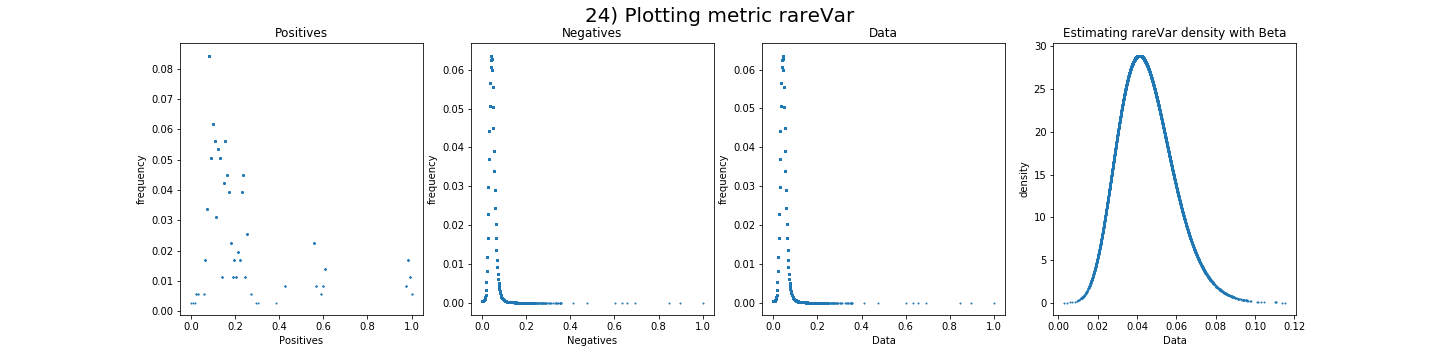
\includegraphics[width=\textwidth]{metrics_statistics/rareVar}
	\caption{Sampling distribution of metric rareVar}
\end{figure}
\subsection{Metric values}
\begin{figure}
	\includegraphics[width=\textwidth]{metrics_plot/rareVar}
	\caption{Values of metric rareVar}
\end{figure}

\clearpage
\section{verPhastCons46way}
\subsection{Metric sample distribution}
The data points seem to follow a \textbf{Gamma} distribution with the following parameters:
\begin{align*}
	\alpha   = 0.4378982063415524    \qquad  \text{loc} = -2.5307968883256733e-31 \qquad \text{scale} = 0.43138079305533483
\end{align*}
\begin{figure}
	\includegraphics[width=\textwidth]{metrics_statistics/verPhastCons46way}
	\caption{Sampling distribution of metric verPhastCons46way}
\end{figure}
\subsection{Metric values}
\begin{figure}
	\includegraphics[width=\textwidth]{metrics_plot/verPhastCons46way}
	\caption{Values of metric verPhastCons46way}
\end{figure}

\clearpage
\section{verPhyloP46way}
\subsection{Metric sample distribution}
The data points seem to follow a \textbf{Gaussian} distribution with the following parameters:

\begin{align*}
	\mean{X} = 0.5723779382558164 & \qquad \Var{X} = 0.0662715947139185
\end{align*}
\begin{figure}
	\includegraphics[width=\textwidth]{metrics_statistics/verPhyloP46way}
	\caption{Sampling distribution of metric verPhyloP46way}
\end{figure}
\subsection{Metric values}
\begin{figure}
	\includegraphics[width=\textwidth]{metrics_plot/verPhyloP46way}
	\caption{Values of metric verPhyloP46way}
\end{figure}

\chapter{Metric distribution summary}
The metrics seem to follow these sample distributions:

\begin{table}
	\begin{tabular}{|l|l|}
		\hline
		\textbf{Metric}     & \textbf{Distribution} \\
		\hline
		CpGobsExp           & Beta                  \\
		\hline
		CpGperCpG           & Beta                  \\
		\hline
		CpGperGC            & Gaussian              \\
		\hline
		DGVCount            & Gamma                 \\
		\hline
		DnaseClusteredHyp   & Gamma                 \\
		\hline
		EncH3K27Ac          & Gamma                 \\
		\hline
		GCContent           & Gaussian              \\
		\hline
		EncH3K4Me3          & Gamma                 \\
		\hline
		ISCApath            & Gamma                 \\
		\hline
		DnaseClusteredScore & Beta                  \\
		\hline
		EncH3K4Me1          & Gamma                 \\
		\hline
		GerpRS              & Gamma                 \\
		\hline
		GerpRSpv            & Gamma                 \\
		\hline
		commonVar           & Exponential Weibull   \\
		\hline
		dbVARCount          & Gamma                 \\
		\hline
		fantom5Perm         & Gamma                 \\
		\hline
		fantom5Robust       & Gamma                 \\
		\hline
		mamPhastCons46way   & Gamma                 \\
		\hline
		priPhastCons46way   & Gamma                 \\
		\hline
		rareVar             & Beta                  \\
		\hline
		verPhastCons46way   & Gamma                 \\
		\hline
		numTFBSConserved    & Exponential           \\
		\hline
		fracRareCommon      & Beta                  \\
		\hline
		priPhyloP46way      & Beta                  \\
		\hline
		verPhyloP46way      & Gaussian              \\
		\hline
		mamPhyloP46way      & Gaussian              \\
		\hline
	\end{tabular}
	\caption{Metrics and their distribution}
\end{table}

\chapter{Scatter plot}
We now proceed to draw a scatter plot trying to identify eventual data correlations.

\section{Scatter plot}
A scatter plot with higher resolution is available in the project repository.
\begin{center}
	\makebox[\textwidth]{
		\includegraphics[width=\paperwidth]{scatter_plot}
	}
\end{center}

\section{Identified data correlations}
Data correlations seem to exist between:

\subsection{dbVARCount and DGVCount}
There is a strong correlation between this two metrics: let's look again at the data plots to see if they follow a similar trend:

\begin{figure}
	\includegraphics[width=\textwidth]{metrics_statistics/dbVARCount}
	\caption{Sampling distribution of metric dbVARCount}
\end{figure}
\begin{figure}
	\includegraphics[width=\textwidth]{metrics_statistics/DGVCount}
	\caption{Sampling distribution of metric DGVCount}
\end{figure}
\begin{figure}
	\includegraphics[width=\textwidth]{metrics_plot/dbVARCount}
	\caption{Values of metric dbVARCount}
\end{figure}
\begin{figure}
	\includegraphics[width=\textwidth]{metrics_plot/DGVCount}
	\caption{Values of metric DGVCount}
\end{figure}

The two metrics seem \textbf{highly} correlated, if not the \textbf{same metric}. This means that one of the two could be removed from the dataset, as it does not add any useful information.

\subsection{mamPhyloP46way and verPhyloP46way}
There is a some correlation between this two metrics: let's look again at the data plots to see if they follow a similar trend:

\begin{figure}
	\includegraphics[width=\textwidth]{metrics_statistics/mamPhyloP46way}
	\caption{Sampling distribution of metric mamPhyloP46way}
\end{figure}
\begin{figure}
	\includegraphics[width=\textwidth]{metrics_statistics/verPhyloP46way}
	\caption{Sampling distribution of metric verPhyloP46way}
\end{figure}
\begin{figure}
	\includegraphics[width=\textwidth]{metrics_plot/mamPhyloP46way}
	\caption{Values of metric mamPhyloP46way}
\end{figure}
\begin{figure}
	\includegraphics[width=\textwidth]{metrics_plot/verPhyloP46way}
	\caption{Values of metric verPhyloP46way}
\end{figure}

The two metrics seem \textbf{slightly} correlated, but not enough to consider removing one of the two.

\part{Theory}
\chapter{Input modelling}

\section{Input values}
The values used for each metric are the 3 following:

\subsection{Normalized metric}
Clearly one of the important metrics is the metric itself, that will be normalized to allow for input in \(\sqr{0,1}\) range:

\begin{figure}
	\[
		\text{metric}' = \frac{\text{metric} - \min\crl{\text{metric values}}}{\max\crl{\text{metric values}}- \min\crl{\text{metric values}}}
	\]
	\caption{Input normalization to \(\sqr{0,1}\) range}
\end{figure}

\subsection{Rarity}
Another value we will be using in the input layer of the network is the rarity of the metric value, modelled as the surprise value of the estimated sampling distribution of the metric:

If \(M\) is the estimated metric distribution cumulative distribution function (CDF), \(m\) is the value assumed by the metric in the given data point and \(\epsilon \) is a range, we can model \textbf{rarity} as follows:
\begin{figure}
	\[
		\prob{m - \epsilon \leq X \leq m + \epsilon} = M(m + \epsilon) - M(m - \epsilon) \qquad \text{rarity}(m) = 1- \prob{m - \epsilon \leq X \leq m + \epsilon}
	\]
	\caption{Rarity}
\end{figure}

\subsection{Entropy}
The third and final value used will be \textbf{entropy}, obtained using the estimated metric probability:

\begin{figure}
	\[
		H(x) = -\prob{m - \epsilon \leq X \leq m + \epsilon}\log\prob{m - \epsilon \leq X \leq m + \epsilon}
	\]
	\caption{Entropy}
\end{figure}

\section{Feet}
The input layer is comprised of 25 (number of metrics, excluded the one recognized to be in strong correlation to another) \textit{feet}, meaning tiny networks that are used to limit the initial linear combination of the metric input values to themselves.

Each feet is modelled as a locally connected dense layer, with a window of 3 neurons.

\section{Oversampling of positives}
Since the positive values are just the \(0.036\% \) of the dataset we'll oversample these to weight more these values. Since the variance of positive data points is too high to extrapolate a distribution to generate significant new fuzzy data points, simple duplication will be used.

\section{Undersampling of negatives}
Since the negative values are more than the \(99.96\% \) of the dataset we'll undersample these to weight less these values.

\section{Oversampling and undersampling targets}
Oversampling and undersampling target will be to have a training dataset with \(1\% \) of positives and \(99\% \) of negatives.

\section{Absence of information}
Absence of information about a given metric will be modelled as \textbf{zeros}, meaning all values relative to the given absent metric for that data point will be treated as zero.

\chapter{Output modelling}
The output layer of the neural network is modelled by \textbf{two} neurons, one representing the positive class and one the negative class, with a \textbf{sigmoid} as activation function.

\chapter{Weight initialization}
\section{Weight distribution based on input distribution}
Since input values are not from any particular distribution or hold properties such as \(\mean{X} = 0\) or \(\Var{X} = 1\) (in some metrics mean and variance are far from these values) they do not suggest to use any specific distribution.

\section{Weight distribution based on activation functions and regularization layers}
The codomain values from the activation functions, being SELU for most of the network, tend to hold the properties of \(\mean{X} = 0\) and \(\Var{X} = 1\) (\url{http://arxiv.org/abs/1706.02515}). These values are then regularized to penalize extreme weights that may appear when variance starts with a value significantly away from \(1\).

For these properties weight will be initialized by extracting them from a Gaussian with \(\mean{X} = 0\) and \(\Var{X} = 1\).

\chapter{Locally connected dense layers}
The first two layers will be locally connected dense layers, to exploit the positional information of the input values.

Other than the group of triples, input will be sorted by distribution kind so that the initial interpolations happen mostly with data from the same distribution family.

\begin{figure}
	\includegraphics[width=0.3\textwidth]{locally_connected}
	\caption{Locally connected layer}
\end{figure}

\section{Activation function}
We'll be using a \textbf{leaky relu} for the locally connected dense layers with \(\alpha=0.3\).

\begin{figure}
	\includegraphics[width=0.8\textwidth]{relu}
	\caption{RELU and Leaky RELU}
\end{figure}

\chapter{Dense layers}
For the following hidden layers we will be using dense connected layers, with a piramidal structure (reducing the number of the neurons from 26 to 2).

\begin{figure}
	\includegraphics[width=0.3\textwidth]{dense_connected}
	\caption{Dense connected layer}
\end{figure}

\section{Activation function}
We'll be using again \textbf{leaky relu} and experimenting with \textbf{SELU} for the dense layers:

\begin{figure}
	\[
		\text{selu}(x) = \lambda \begin{cases}
			x                 & x > 0    \\
			\alpha e^x-\alpha & x \leq 0
		\end{cases}
	\]
	\caption{SELU}
\end{figure}

\section{Regularization}
Regularization layers will be alternated to the dense layers to penalize weight extreme growth.

\section{Drop out}
In addition to regularization, also \textbf{drop out} of \(10\% \) of neurons per hidden layer will be applied.

\input{\main/../../general/footer.tex}

\chapter{References}
LatexTools does not compile references at this time.

\end{document}
\addbibresource{references.bib}

\bash{mkdir tikz}
\tikzexternalize[prefix=tikz/]

\usepackage{booktabs}
\begin{document}

\hypersetup{pageanchor=false}
\begin{titlepage}
	\begin{center}
		\ifLuaTeX
			\directlua{dofile(deapness.."/general/lua/title.lua")}
		\else
			\large{TITLEPAGE NOT RENDERED!\\RECOMPILE WITH LUATEX!}
		\fi
	\end{center}
\end{titlepage}
\hypersetup{pageanchor=true}

{\hypersetup{hidelinks}
	\tableofcontents  % Generates the table of contents
}
\part{Dataset}
\chapter{Data points}
First we begin looking at the dataset, the distributions of the given metrics and the statistical analysis of these data points.

\section{Retrieving the dataset}
The dataset can be downloaded from \url{https://homes.di.unimi.it/valentini/ProgettoBioinformatica1718/data/}.

\section{Composition}
\subsection{Training dataset}
In the training dataset there are 981389 data points, each one comprised of 26 metrics. The first 356 are pathogenic and all the others are negative.

\subsection{Testing dataset}
In the test dataset there are 190189 data points, still each one comprised of 26 metrics. The first 40 are pathogenic and the following are negative.

\chapter{Metrics}
\section{How the graphs are realized}
All the graphs are in triples: positives, negatives and mixed. All the zeros are removed as in most metrics \textit{seemed} to indicate an unknown value.

\subsection{Metric sample distribution}
Are realized by calculating the frequencies and estimating the density distributions parameters via MLE.

\subsection{Plot graphs}
Are realized by sorting the values of the metric.

\subsection{Normalized plot graphs}
Are realized by sorting the values of the metric, with the domain and codomain normalized.

\clearpage
\section{CpGobsExp}
\subsection{Metric sample distribution}
The data points seem to follow a \textbf{Beta} distribution with the following parameters:

\begin{align*}
	\alpha   = 7.6689746880295795     & \qquad  \beta = 6778383.524935903       \\
	\text{loc} = -0.09826818916997124 & \qquad \text{scale} = 306278.3184506849
\end{align*}

\begin{figure}
	\includegraphics[width=\textwidth]{metrics_statistics/CpGobsExp}
	\caption{Sampling distribution of metric CpGobsExp}
\end{figure}
\subsection{Metric values}
\begin{figure}
	\includegraphics[width=\textwidth]{metrics_plot/CpGobsExp}
	\caption{Values of metric CpGobsExp}
\end{figure}

\clearpage
\section{CpGperCpG}
\subsection{Metric sample distribution}
The data points seem to follow a \textbf{Beta} distribution with the following parameters:

\begin{align*}
	\alpha   = 6.402175341881067      & \qquad  \beta = 97129163.31117742      \\
	\text{loc} = -0.05698922703576313 & \qquad \text{scale} = 4337764.42876015
\end{align*}
\begin{figure}
	\includegraphics[width=\textwidth]{metrics_statistics/CpGperCpG}
	\caption{Sampling distribution of metric CpGperCpG}
\end{figure}
\subsection{Metric values}
\begin{figure}
	\includegraphics[width=\textwidth]{metrics_plot/CpGperCpG}
	\caption{Values of metric CpGperCpG}
\end{figure}

\clearpage
\section{CpGperGC}
\subsection{Metric sample distribution}
The data points seem to follow a \textbf{Gaussian} distribution with the following parameters:

\begin{align*}
	\mean{X} = 0.4602356242601636 & \qquad \Var{X} = 0.15949294643574352
\end{align*}
\begin{figure}
	\includegraphics[width=\textwidth]{metrics_statistics/CpGperGC}
	\caption{Sampling distribution of metric CpGperGC}
\end{figure}
\subsection{Metric values}
\begin{figure}
	\includegraphics[width=\textwidth]{metrics_plot/CpGperGC}
	\caption{Values of metric CpGperGC}
\end{figure}

\clearpage
\section{DGVCount}
\subsection{Metric sample distribution}
The data points seem to follow a \textbf{Gamma} distribution with the following parameters:
\begin{align*}
	\alpha   = 0.20940038672579409    \qquad  \text{loc} = -1.1962983066939984e-30 \qquad \text{scale} = 1.2347090894162929
\end{align*}
\begin{figure}
	\includegraphics[width=\textwidth]{metrics_statistics/DGVCount}
	\caption{Sampling distribution of metric DGVCount}
\end{figure}
\subsection{Metric values}
\begin{figure}
	\includegraphics[width=\textwidth]{metrics_plot/DGVCount}
	\caption{Values of metric DGVCount}
\end{figure}

\clearpage
\section{DnaseClusteredHyp}
\subsection{Metric sample distribution}
The data points seem to follow a \textbf{Gamma} distribution with the following parameters:
\begin{align*}
	\alpha   = 0.4176887081406805    \qquad  \text{loc} = -3.362626207862299e-29 \qquad \text{scale} = 0.3676310948709975
\end{align*}
\begin{figure}
	\includegraphics[width=\textwidth]{metrics_statistics/DnaseClusteredHyp}
	\caption{Sampling distribution of metric DnaseClusteredHyp}
\end{figure}
\subsection{Metric values}
\begin{figure}
	\includegraphics[width=\textwidth]{metrics_plot/DnaseClusteredHyp}
	\caption{Values of metric DnaseClusteredHyp}
\end{figure}

\clearpage
\section{DnaseClusteredScore}
\subsection{Metric sample distribution}
The data points seem to follow \textbf{slightly} a \textbf{Beta} distribution with the following parameters:
\begin{align*}
	\alpha   = 0.2709657632937803     & \qquad  \beta = 0.44530002562349713      \\
	\text{loc} = -0.09309893086089688 & \qquad \text{scale} = 1.0930989308608972
\end{align*}

\begin{figure}
	\includegraphics[width=\textwidth]{metrics_statistics/DnaseClusteredScore}
	\caption{Sampling distribution of metric DnaseClusteredScore}
\end{figure}
\subsection{Metric values}
\begin{figure}
	\includegraphics[width=\textwidth]{metrics_plot/DnaseClusteredScore}
	\caption{Values of metric DnaseClusteredScore}
\end{figure}

\clearpage
\section{EncH3K27Ac}
\subsection{Metric sample distribution}
The data points seem to follow a family of \textbf{Gamma} distributions (a speculation for this distribution could be the different groups from which the data are extracted), we will approximate them to one with a linear combination of the parameters:
\begin{align*}
	\alpha   = 0.0004042086221537893    \qquad  \text{loc} = -2.859398162696207e-24 \qquad \text{scale} = 0.03076944787133299
\end{align*}
\begin{figure}
	\includegraphics[width=\textwidth]{metrics_statistics/EncH3K27Ac}
	\caption{Sampling distribution of metric EncH3K27Ac}
\end{figure}
\subsection{Metric values}
\begin{figure}
	\includegraphics[width=\textwidth]{metrics_plot/EncH3K27Ac}
	\caption{Values of metric EncH3K27Ac}
\end{figure}

\clearpage
\section{EncH3K4Me1}
\subsection{Metric sample distribution}
The data points seem to follow a family of \textbf{Gamma} distributions (a speculation for this distribution could be the different groups from which the data are extracted), we will approximate them to one with a linear combination of the parameters:
\begin{align*}
	\alpha   = 0.22566387737236238    \qquad  \text{loc} = -6.619765504581537e-27 \qquad \text{scale} = 1.396157055181753
\end{align*}
\begin{figure}
	\includegraphics[width=\textwidth]{metrics_statistics/EncH3K4Me1}
	\caption{Sampling distribution of metric EncH3K4Me1}
\end{figure}
\subsection{Metric values}
\begin{figure}
	\includegraphics[width=\textwidth]{metrics_plot/EncH3K4Me1}
	\caption{Values of metric EncH3K4Me1}
\end{figure}

\clearpage
\section{EncH3K4Me3}
\subsection{Metric sample distribution}
The data points seem to follow a family of \textbf{Gamma} distributions (a speculation for this distribution could be the different groups from which the data are extracted), we will approximate them to one with a linear combination of the parameters:
\begin{align*}
	\alpha   = 0.007502428717446465    \qquad  \text{loc} = -3.469650119186857e-25 \qquad \text{scale} = 0.04125297431971783
\end{align*}
\begin{figure}
	\includegraphics[width=\textwidth]{metrics_statistics/EncH3K4Me3}
	\caption{Sampling distribution of metric EncH3K4Me3}
\end{figure}
\subsection{Metric values}
\begin{figure}
	\includegraphics[width=\textwidth]{metrics_plot/EncH3K4Me3}
	\caption{Values of metric EncH3K4Me3}
\end{figure}

\clearpage
\section{GCContent}
\subsection{Metric sample distribution}
The data points seem to be a combination of two \textbf{Gaussian} distributions. This will be approximated to one with the following parameters:

\begin{align*}
	\mean{X} = 0.4482813176478024 & \qquad \Var{X} = 0.1097424869360011
\end{align*}
\begin{figure}
	\includegraphics[width=\textwidth]{metrics_statistics/GCContent}
	\caption{Sampling distribution of metric GCContent}
\end{figure}
\subsection{Metric values}
\begin{figure}
	\includegraphics[width=\textwidth]{metrics_plot/GCContent}
	\caption{Values of metric GCContent}
\end{figure}

\clearpage
\section{GerpRS}
\subsection{Metric sample distribution}
The data points seem to follow a family of \textbf{Gamma} distributions (a speculation for this distribution could be the different groups from which the data are extracted), we will approximate them to one with a linear combination of the parameters:
\begin{align*}
	\alpha   = 0.8688332877203315    \qquad  \text{loc} = -1.7081810436826354e-28 \qquad \text{scale} = 0.11512094125204281
\end{align*}
\begin{figure}
	\includegraphics[width=\textwidth]{metrics_statistics/GerpRS}
	\caption{Sampling distribution of metric GerpRS}
\end{figure}
\subsection{Metric values}
\begin{figure}
	\includegraphics[width=\textwidth]{metrics_plot/GerpRS}
	\caption{Values of metric GerpRS}
\end{figure}

\clearpage
\section{GerpRSpv}
\subsection{Metric sample distribution}
The data points seem to follow a family of \textbf{Gamma} distributions (a speculation for this distribution could be the different groups from which the data are extracted), we will approximate them to one with a linear combination of the parameters:
\begin{align*}
	\alpha   = 0.5165290213220888    \qquad  \text{loc} = -6.952792177974854e-30 \qquad \text{scale} = 0.2530358950266992
\end{align*}
\begin{figure}
	\includegraphics[width=\textwidth]{metrics_statistics/GerpRSpv}
	\caption{Sampling distribution of metric GerpRSpv}
\end{figure}
\subsection{Metric values}
\begin{figure}
	\includegraphics[width=\textwidth]{metrics_plot/GerpRSpv}
	\caption{Values of metric GerpRSpv}
\end{figure}

\clearpage
\section{ISCApath}
\subsection{Metric sample distribution}
The data points seem to follow a \textbf{Gamma} distribution with the following parameters:
\begin{align*}
	\alpha   = 0.08318618903703257    \qquad  \text{loc} = -1.9358902729364646e-30 \qquad \text{scale} = 1.2606790181148981
\end{align*}
\begin{figure}
	\includegraphics[width=\textwidth]{metrics_statistics/ISCApath}
	\caption{Sampling distribution of metric ISCApath}
\end{figure}
\subsection{Metric values}
\begin{figure}
	\includegraphics[width=\textwidth]{metrics_plot/ISCApath}
	\caption{Values of metric ISCApath}
\end{figure}

\clearpage
\section{commonVar}
\subsection{Metric sample distribution}
The data points seem to follow an \textbf{Exponential Weibull} distribution with the following parameters:

\begin{align*}
	\alpha   = 5.038707296051438       & \qquad  \beta = 1.0160276119461702         \\
	\text{loc} = -0.012528678364149837 & \qquad \text{scale} = 0.025052745155722922
\end{align*}
\begin{figure}
	\includegraphics[width=\textwidth]{metrics_statistics/commonVar}
	\caption{Sampling distribution of metric commonVar}
\end{figure}
\subsection{Metric values}
\begin{figure}
	\includegraphics[width=\textwidth]{metrics_plot/commonVar}
	\caption{Values of metric commonVar}
\end{figure}

\clearpage
\section{dbVARCount}
\subsection{Metric sample distribution}
The data points seem to follow a \textbf{Gamma} distribution with the following parameters:
\begin{align*}
	\alpha   = 0.20940038672579409    \qquad  \text{loc} = -1.1962983066939984e-30 \qquad \text{scale} = 1.2347090894162929
\end{align*}
\begin{figure}
	\includegraphics[width=\textwidth]{metrics_statistics/dbVARCount}
	\caption{Sampling distribution of metric dbVARCount}
\end{figure}
\subsection{Metric values}
\begin{figure}
	\includegraphics[width=\textwidth]{metrics_plot/dbVARCount}
	\caption{Values of metric dbVARCount}
\end{figure}

\clearpage
\section{fantom5Perm}
\subsection{Metric sample distribution}
The data points seem to follow a \textbf{Gamma} distribution with the following parameters:
\begin{align*}
	\alpha   = 0.06895533706017208    \qquad  \text{loc} = -3.220296247423778e-30 \qquad \text{scale} = 1.2605014923175824
\end{align*}
\begin{figure}
	\includegraphics[width=\textwidth]{metrics_statistics/fantom5Perm}
	\caption{Sampling distribution of metric fantom5Perm}
\end{figure}
\subsection{Metric values}
\begin{figure}
	\includegraphics[width=\textwidth]{metrics_plot/fantom5Perm}
	\caption{Values of metric fantom5Perm}
\end{figure}

\clearpage
\section{fantom5Robust}
\subsection{Metric sample distribution}
The data points seem to follow a \textbf{Gamma} distribution with the following parameters:
\begin{align*}
	\alpha   = 0.08983952110680529    \qquad  \text{loc} = -3.220296247423778e-30 \qquad \text{scale} = 1.2605014923175824
\end{align*}
\begin{figure}
	\includegraphics[width=\textwidth]{metrics_statistics/fantom5Robust}
	\caption{Sampling distribution of metric fantom5Robust}
\end{figure}
\subsection{Metric values}
\begin{figure}
	\includegraphics[width=\textwidth]{metrics_plot/fantom5Robust}
	\caption{Values of metric fantom5Robust}
\end{figure}

\clearpage
\section{fracRareCommon}
\subsection{Metric sample distribution}
The data points seem to follow an \textbf{Beta} distribution with the following parameters:

\begin{align*}
	\alpha   = 2772.739504773501    & \qquad  \beta = 14.986077009876375      \\
	\text{loc} = -69.93503912437342 & \qquad \text{scale} = 71.09741090721741
\end{align*}
\begin{figure}
	\includegraphics[width=\textwidth]{metrics_statistics/fracRareCommon}
	\caption{Sampling distribution of metric fracRareCommon}
\end{figure}
\subsection{Metric values}
\begin{figure}
	\includegraphics[width=\textwidth]{metrics_plot/fracRareCommon}
	\caption{Values of metric fracRareCommon}
\end{figure}

\clearpage
\section{mamPhastCons46way}
\subsection{Metric sample distribution}
The data points seem to follow a \textbf{Gamma} distribution with the following parameters:
\begin{align*}
	\alpha   = 0.3215099801387991    \qquad  \text{loc} = -6.260887365023215e-31 \qquad \text{scale} = 0.45230902834164866
\end{align*}
\begin{figure}
	\includegraphics[width=\textwidth]{metrics_statistics/mamPhastCons46way}
	\caption{Sampling distribution of metric mamPhastCons46way}
\end{figure}
\subsection{Metric values}
\begin{figure}
	\includegraphics[width=\textwidth]{metrics_plot/mamPhastCons46way}
	\caption{Values of metric mamPhastCons46way}
\end{figure}

\clearpage
\section{mamPhyloP46way}
\subsection{Metric sample distribution}
The data points seem to follow a \textbf{Gaussian} distribution with the following parameters:

\begin{align*}
	\mean{X} = 0.7032457913828309 & \qquad \Var{X} = 0.07627203289198752
\end{align*}
\begin{figure}
	\includegraphics[width=\textwidth]{metrics_statistics/mamPhyloP46way}
	\caption{Sampling distribution of metric mamPhyloP46way}
\end{figure}
\subsection{Metric values}
\begin{figure}
	\includegraphics[width=\textwidth]{metrics_plot/mamPhyloP46way}
	\caption{Values of metric mamPhyloP46way}
\end{figure}

\clearpage
\section{numTFBSConserved}
\subsection{Metric sample distribution}
The data points seem to follow a \textbf{exponential} distribution with the following parameters:

\begin{align*}
	\mean{X} = -4.600037873301623e-12 & \qquad \Var{X} = 0.033419421646804975
\end{align*}
\begin{figure}
	\includegraphics[width=\textwidth]{metrics_statistics/numTFBSConserved}
	\caption{Sampling distribution of metric numTFBSConserved}
\end{figure}
\subsection{Metric values}
\begin{figure}
	\includegraphics[width=\textwidth]{metrics_plot/numTFBSConserved}
	\caption{Values of metric numTFBSConserved}
\end{figure}

\clearpage
\section{priPhastCons46way}
\subsection{Metric sample distribution}
The data points seem to follow a \textbf{Gamma} distribution with the following parameters:
\begin{align*}
	\alpha   = 0.2836383862597563    \qquad  \text{loc} = -1.8643137904859329e-31 \qquad \text{scale} = 0.37399746075497264
\end{align*}
\begin{figure}
	\includegraphics[width=\textwidth]{metrics_statistics/priPhastCons46way}
	\caption{Sampling distribution of metric priPhastCons46way}
\end{figure}
\subsection{Metric values}
\begin{figure}
	\includegraphics[width=\textwidth]{metrics_plot/priPhastCons46way}
	\caption{Values of metric priPhastCons46way}
\end{figure}

\clearpage
\section{priPhyloP46way}
\subsection{Metric sample distribution}
The data points seem to follow an \textbf{Beta} distribution with the following parameters:

\begin{align*}
	\alpha   = 2095270.7440875275    & \qquad  \beta = 4.199025269606416        \\
	\text{loc} = -103376.03746996864 & \qquad \text{scale} = 103377.03863437689
\end{align*}
\begin{figure}
	\includegraphics[width=\textwidth]{metrics_statistics/priPhyloP46way}
	\caption{Sampling distribution of metric priPhyloP46way}
\end{figure}
\subsection{Metric values}
\begin{figure}
	\includegraphics[width=\textwidth]{metrics_plot/priPhyloP46way}
	\caption{Values of metric priPhyloP46way}
\end{figure}

\clearpage
\section{rareVar}
\subsection{Metric sample distribution}
The data points seem to follow an \textbf{Beta} distribution with the following parameters:

\begin{align*}
	\alpha   = 14.148202647100376      & \qquad  \beta = 7669045.025220526        \\
	\text{loc} = -0.008523116473417407 & \qquad \text{scale} = 28973.953544984728
\end{align*}
\begin{figure}
	\includegraphics[width=\textwidth]{metrics_statistics/rareVar}
	\caption{Sampling distribution of metric rareVar}
\end{figure}
\subsection{Metric values}
\begin{figure}
	\includegraphics[width=\textwidth]{metrics_plot/rareVar}
	\caption{Values of metric rareVar}
\end{figure}

\clearpage
\section{verPhastCons46way}
\subsection{Metric sample distribution}
The data points seem to follow a \textbf{Gamma} distribution with the following parameters:
\begin{align*}
	\alpha   = 0.4378982063415524    \qquad  \text{loc} = -2.5307968883256733e-31 \qquad \text{scale} = 0.43138079305533483
\end{align*}
\begin{figure}
	\includegraphics[width=\textwidth]{metrics_statistics/verPhastCons46way}
	\caption{Sampling distribution of metric verPhastCons46way}
\end{figure}
\subsection{Metric values}
\begin{figure}
	\includegraphics[width=\textwidth]{metrics_plot/verPhastCons46way}
	\caption{Values of metric verPhastCons46way}
\end{figure}

\clearpage
\section{verPhyloP46way}
\subsection{Metric sample distribution}
The data points seem to follow a \textbf{Gaussian} distribution with the following parameters:

\begin{align*}
	\mean{X} = 0.5723779382558164 & \qquad \Var{X} = 0.0662715947139185
\end{align*}
\begin{figure}
	\includegraphics[width=\textwidth]{metrics_statistics/verPhyloP46way}
	\caption{Sampling distribution of metric verPhyloP46way}
\end{figure}
\subsection{Metric values}
\begin{figure}
	\includegraphics[width=\textwidth]{metrics_plot/verPhyloP46way}
	\caption{Values of metric verPhyloP46way}
\end{figure}

\chapter{Metric distribution summary}
The metrics seem to follow these sample distributions:

\begin{table}
	\begin{tabular}{|l|l|}
		\hline
		\textbf{Metric}     & \textbf{Distribution} \\
		\hline
		CpGobsExp           & Beta                  \\
		\hline
		CpGperCpG           & Beta                  \\
		\hline
		CpGperGC            & Gaussian              \\
		\hline
		DGVCount            & Gamma                 \\
		\hline
		DnaseClusteredHyp   & Gamma                 \\
		\hline
		EncH3K27Ac          & Gamma                 \\
		\hline
		GCContent           & Gaussian              \\
		\hline
		EncH3K4Me3          & Gamma                 \\
		\hline
		ISCApath            & Gamma                 \\
		\hline
		DnaseClusteredScore & Beta                  \\
		\hline
		EncH3K4Me1          & Gamma                 \\
		\hline
		GerpRS              & Gamma                 \\
		\hline
		GerpRSpv            & Gamma                 \\
		\hline
		commonVar           & Exponential Weibull   \\
		\hline
		dbVARCount          & Gamma                 \\
		\hline
		fantom5Perm         & Gamma                 \\
		\hline
		fantom5Robust       & Gamma                 \\
		\hline
		mamPhastCons46way   & Gamma                 \\
		\hline
		priPhastCons46way   & Gamma                 \\
		\hline
		rareVar             & Beta                  \\
		\hline
		verPhastCons46way   & Gamma                 \\
		\hline
		numTFBSConserved    & Exponential           \\
		\hline
		fracRareCommon      & Beta                  \\
		\hline
		priPhyloP46way      & Beta                  \\
		\hline
		verPhyloP46way      & Gaussian              \\
		\hline
		mamPhyloP46way      & Gaussian              \\
		\hline
	\end{tabular}
	\caption{Metrics and their distribution}
\end{table}

\chapter{Scatter plot}
We now proceed to draw a scatter plot trying to identify eventual data correlations.

\section{Scatter plot}
A scatter plot with higher resolution is available in the project repository.
\begin{center}
	\makebox[\textwidth]{
		\includegraphics[width=\paperwidth]{scatter_plot}
	}
\end{center}

\section{Identified data correlations}
Data correlations seem to exist between:

\subsection{dbVARCount and DGVCount}
There is a strong correlation between this two metrics: let's look again at the data plots to see if they follow a similar trend:

\begin{figure}
	\includegraphics[width=\textwidth]{metrics_statistics/dbVARCount}
	\caption{Sampling distribution of metric dbVARCount}
\end{figure}
\begin{figure}
	\includegraphics[width=\textwidth]{metrics_statistics/DGVCount}
	\caption{Sampling distribution of metric DGVCount}
\end{figure}
\begin{figure}
	\includegraphics[width=\textwidth]{metrics_plot/dbVARCount}
	\caption{Values of metric dbVARCount}
\end{figure}
\begin{figure}
	\includegraphics[width=\textwidth]{metrics_plot/DGVCount}
	\caption{Values of metric DGVCount}
\end{figure}

The two metrics seem \textbf{highly} correlated, if not the \textbf{same metric}. This means that one of the two could be removed from the dataset, as it does not add any useful information.

\subsection{mamPhyloP46way and verPhyloP46way}
There is a some correlation between this two metrics: let's look again at the data plots to see if they follow a similar trend:

\begin{figure}
	\includegraphics[width=\textwidth]{metrics_statistics/mamPhyloP46way}
	\caption{Sampling distribution of metric mamPhyloP46way}
\end{figure}
\begin{figure}
	\includegraphics[width=\textwidth]{metrics_statistics/verPhyloP46way}
	\caption{Sampling distribution of metric verPhyloP46way}
\end{figure}
\begin{figure}
	\includegraphics[width=\textwidth]{metrics_plot/mamPhyloP46way}
	\caption{Values of metric mamPhyloP46way}
\end{figure}
\begin{figure}
	\includegraphics[width=\textwidth]{metrics_plot/verPhyloP46way}
	\caption{Values of metric verPhyloP46way}
\end{figure}

The two metrics seem \textbf{slightly} correlated, but not enough to consider removing one of the two.

\part{Theory}
\chapter{Input modelling}

\section{Input values}
The values used for each metric are the 3 following:

\subsection{Normalized metric}
Clearly one of the important metrics is the metric itself, that will be normalized to allow for input in \(\sqr{0,1}\) range:

\begin{figure}
	\[
		\text{metric}' = \frac{\text{metric} - \min\crl{\text{metric values}}}{\max\crl{\text{metric values}}- \min\crl{\text{metric values}}}
	\]
	\caption{Input normalization to \(\sqr{0,1}\) range}
\end{figure}

\subsection{Rarity}
Another value we will be using in the input layer of the network is the rarity of the metric value, modelled as the surprise value of the estimated sampling distribution of the metric:

If \(M\) is the estimated metric distribution cumulative distribution function (CDF), \(m\) is the value assumed by the metric in the given data point and \(\epsilon \) is a range, we can model \textbf{rarity} as follows:
\begin{figure}
	\[
		\prob{m - \epsilon \leq X \leq m + \epsilon} = M(m + \epsilon) - M(m - \epsilon) \qquad \text{rarity}(m) = 1- \prob{m - \epsilon \leq X \leq m + \epsilon}
	\]
	\caption{Rarity}
\end{figure}

\subsection{Entropy}
The third and final value used will be \textbf{entropy}, obtained using the estimated metric probability:

\begin{figure}
	\[
		H(x) = -\prob{m - \epsilon \leq X \leq m + \epsilon}\log\prob{m - \epsilon \leq X \leq m + \epsilon}
	\]
	\caption{Entropy}
\end{figure}

\section{Feet}
The input layer is comprised of 25 (number of metrics, excluded the one recognized to be in strong correlation to another) \textit{feet}, meaning tiny networks that are used to limit the initial linear combination of the metric input values to themselves.

Each feet is modelled as a locally connected dense layer, with a window of 3 neurons.

\section{Oversampling of positives}
Since the positive values are just the \(0.036\% \) of the dataset we'll oversample these to weight more these values. Since the variance of positive data points is too high to extrapolate a distribution to generate significant new fuzzy data points, simple duplication will be used.

\section{Undersampling of negatives}
Since the negative values are more than the \(99.96\% \) of the dataset we'll undersample these to weight less these values.

\section{Oversampling and undersampling targets}
Oversampling and undersampling target will be to have a training dataset with \(1\% \) of positives and \(99\% \) of negatives.

\section{Absence of information}
Absence of information about a given metric will be modelled as \textbf{zeros}, meaning all values relative to the given absent metric for that data point will be treated as zero.

\chapter{Output modelling}
The output layer of the neural network is modelled by \textbf{two} neurons, one representing the positive class and one the negative class, with a \textbf{sigmoid} as activation function.

\chapter{Weight initialization}
\section{Weight distribution based on input distribution}
Since input values are not from any particular distribution or hold properties such as \(\mean{X} = 0\) or \(\Var{X} = 1\) (in some metrics mean and variance are far from these values) they do not suggest to use any specific distribution.

\section{Weight distribution based on activation functions and regularization layers}
The codomain values from the activation functions, being SELU for most of the network, tend to hold the properties of \(\mean{X} = 0\) and \(\Var{X} = 1\) (\url{http://arxiv.org/abs/1706.02515}). These values are then regularized to penalize extreme weights that may appear when variance starts with a value significantly away from \(1\).

For these properties weight will be initialized by extracting them from a Gaussian with \(\mean{X} = 0\) and \(\Var{X} = 1\).

\chapter{Locally connected dense layers}
The first two layers will be locally connected dense layers, to exploit the positional information of the input values.

Other than the group of triples, input will be sorted by distribution kind so that the initial interpolations happen mostly with data from the same distribution family.

\begin{figure}
	\includegraphics[width=0.3\textwidth]{locally_connected}
	\caption{Locally connected layer}
\end{figure}

\section{Activation function}
We'll be using a \textbf{leaky relu} for the locally connected dense layers with \(\alpha=0.3\).

\begin{figure}
	\includegraphics[width=0.8\textwidth]{relu}
	\caption{RELU and Leaky RELU}
\end{figure}

\chapter{Dense layers}
For the following hidden layers we will be using dense connected layers, with a piramidal structure (reducing the number of the neurons from 26 to 2).

\begin{figure}
	\includegraphics[width=0.3\textwidth]{dense_connected}
	\caption{Dense connected layer}
\end{figure}

\section{Activation function}
We'll be using again \textbf{leaky relu} and experimenting with \textbf{SELU} for the dense layers:

\begin{figure}
	\[
		\text{selu}(x) = \lambda \begin{cases}
			x                 & x > 0    \\
			\alpha e^x-\alpha & x \leq 0
		\end{cases}
	\]
	\caption{SELU}
\end{figure}

\section{Regularization}
Regularization layers will be alternated to the dense layers to penalize weight extreme growth.

\section{Drop out}
In addition to regularization, also \textbf{drop out} of \(10\% \) of neurons per hidden layer will be applied.

\printindex

\printglossary

% \printbibliography

\chapter{References}
LatexTools does not compile references at this time.

\end{document}